%%%%%%%%%%%%%%%%%%%%%%%%%%%%%%%%%%%%%%%%%%%%%%%%%%
\begin{frame}[fragile]{Overview}

\begin{itemize}
\item Introduction
\item Event Sourcing 101
\item Homomorphic Event Sourcing
\item Implementation
\item Conclusion
\end{itemize}

\end{frame}

%%%%%%%%%%%%%%%%%%%%%%%%%%%%%%%%%%%%%%%%%%%%%%%%%%
\part{Introduction}

\begin{frame}[fragile]{Why?}

\begin{center}
{
\LARGE
Why?
}

\vspace{2em}

or:

\vspace{2em}

{
\Large
How this all began
}
\end{center}
\end{frame}


\begin{frame}[fragile]{Who?}

\begin{center}
{
\LARGE
Who we are?
}

\vspace{2em}
\end{center}
\end{frame}


\begin{frame}[fragile]{What?}

\begin{center}
{
\LARGE
Trying to integrate formal methods
\\[2em]
Languages, Type Systems, \\[.2em] Engineering Techniques
}

\vspace{2em}
\end{center}
\end{frame}

%%%%%%%%%%%%%%%%%%%%%%%%%%%%%%%%%%%%%%%%%%%%%%%%%%
\part{Event Sourcing 101}

\begin{frame}[fragile]{Ubiquitous Language}

  \begin{itemize}[<+->]
	\item Is $\ldots$ well $\ldots$ ubiquitous
	\item Carries the business language into the code and beyond
	\item Allows everybody to understand everybody else
	\item Understanding without (even unconscious) translation steps
	\item Should be made explicit in a glossary
  \end{itemize}

\end{frame}

\begin{frame}[fragile]{Commands and Events}

  \begin{itemize}[<+->]
  \item Commands represent interactions from the outside world
  \item They are requests to the application
  \item Events  are the system's replies
  \item Events are persistently stored
  \item The current state of the system is the result of all events that happened so far
  \end{itemize}
\end{frame}

\begin{frame}[fragile]{Base Event Loop}
\begin{center}
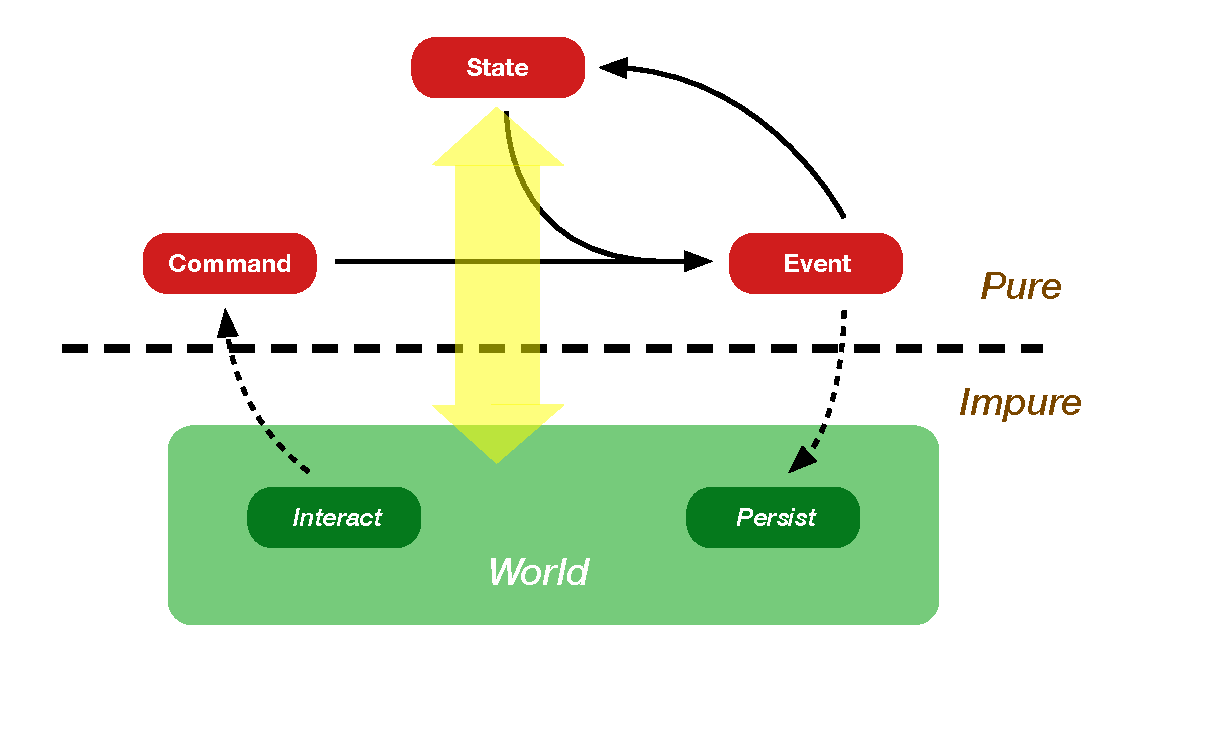
\includegraphics[width=\textwidth]{./images/event-loop.pdf}
\end{center}
\end{frame}

\begin{frame}[fragile]{Event Sourcing as a Formal Language}

\begin{itemize}[<+->]
\item Conceptually, the events comprise a so-called \textit{alphabet}.
\item A \textit{word} is a sequence of letters of this alphabet (i.e.~events).
\item The set of all possible words is a \textit{language}.
\item This means each word of the language corresponds to a \textit{state} of the system.
\item So all the possible states of the system form the language.
\end{itemize}

\end{frame}

%%%%%%%%%%%%%%%%%%%%%%%%%%%%%%%%%%%%%%%%%%%%%%%%%%
\part{Homomorphic Event Sourcing}

\begin{frame}[fragile]{Interacting Components}
\begin{center}
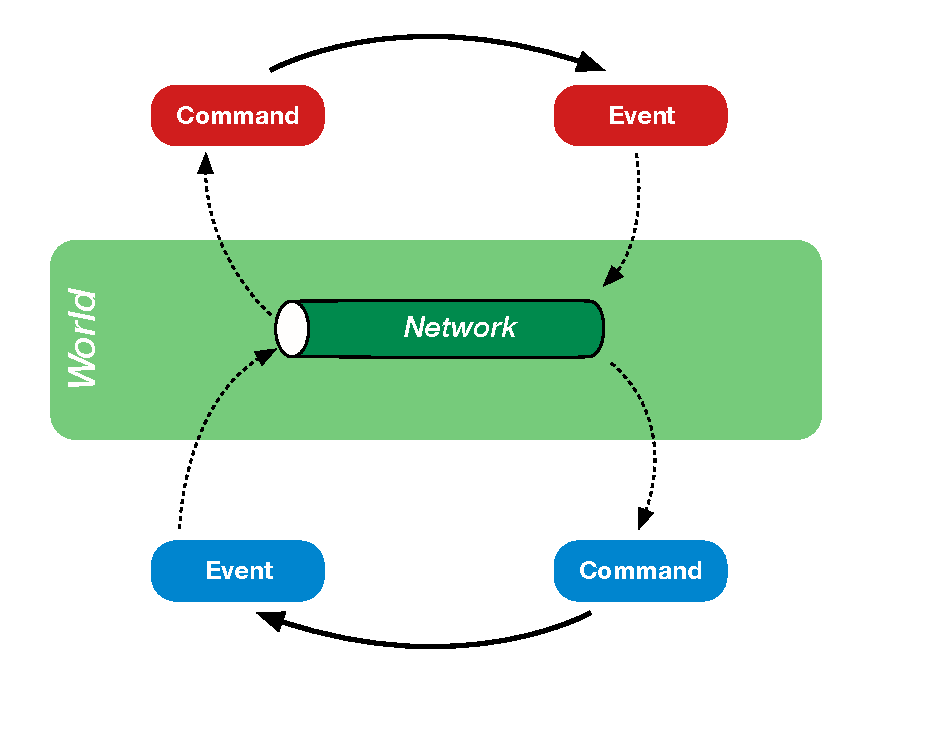
\includegraphics[height=.8\textheight]{./images/interaction-loop.pdf}
\end{center}
\end{frame}

\begin{frame}[fragile]{Interacting Components}
  \begin{itemize}
  \item What happens when 2 event-sourced components have to interact?
  \item We want to map commands to commands and events to events
  \end{itemize}
\end{frame}


\begin{frame}[fragile]{Homomorphism}

  A \emph{homomorphism} is a structure-preserving map between two languages.
   \\[2em]

  \onslide<2->
  This practically means it is enough to
  define a \emph{map} from letters of one language to letters of the other.

\end{frame}

\begin{frame}[fragile]{Homomorphic Event Sourcing}
  \begin{itemize}[<+->]
  \item Define mappings from UI commands to backend commands: A command
    can map to nothing meaning there is no interaction with
    the backend
  \item Define mappings from backend events to UI events: Describes how
    backend's replies are interpreted in the UI
  \item Strive to define \emph{identities}, e.g.~use the same language of commands and events in the frontend and the backend
  \end{itemize}
\end{frame}

%%%%%%%%%%%%%%%%%%%%%%%%%%%%%%%%%%%%%%%%%%%%%%%%%%
\part{Consumer-Driven Contract Testing}

%%%%%%%%%%%%%%%%%%%%%%%%%%%%%%%%%%%%%%%%%%%%%%%%%%
\begin{frame}[fragile]{Standard Problem for Webapps?}

\begin{itemize}
\item Testing that frontend and backend play nicely together
\end{itemize}

\end{frame}

%%%%%%%%%%%%%%%%%%%%%%%%%%%%%%%%%%%%%%%%%%%%%%%%%%
\begin{frame}[fragile]{Standard Approach: ``Super-Na\"ive''}

\only<1>{
\begin{itemize}
\item Backend designs API
\item Backend is developed, tests are written
\item Frontend waits until backend is implemented
\item Frontend is developed
\item Tests for frontend are written
\item Interaction is tested via integration tests
\end{itemize}
}

\only<2>{
Problems:

\begin{itemize}
\item Frontend development is blocked
\item Integration tests are slow
\item Full integration testing does not scale
\end{itemize}
}

\end{frame}

%%%%%%%%%%%%%%%%%%%%%%%%%%%%%%%%%%%%%%%%%%%%%%%%%%
\begin{frame}[fragile]{Standard Approach: ``Still Quite Na\"ive''}

\only<1>{
\begin{itemize}
\item Backend designs API
\item Frontend writes mocks for backend API
\item Backend is developed, tests are written
\item Frontend can also be developed immediately
\item Interaction tests for frontend use these mocks
\end{itemize}
}

\only<2>{
Problems:

\begin{itemize}
\item Frontend relies on mocks for backend API
\item Do the mocks reflect the backend's actual behaviour?
\item Usually, backend behaviour changes
\item Frontend does not notice because mocks still look good
\end{itemize}
}

\end{frame}

%%%%%%%%%%%%%%%%%%%%%%%%%%%%%%%%%%%%%%%%%%%%%%%%%%
\begin{frame}[fragile]{Standard ``Industry-Strength'' Approach}

\only<1>{
\begin{itemize}
\item Consumer-Driven Contract Testing
\item Hand-written contracts
\end{itemize}
}

\only<2>{
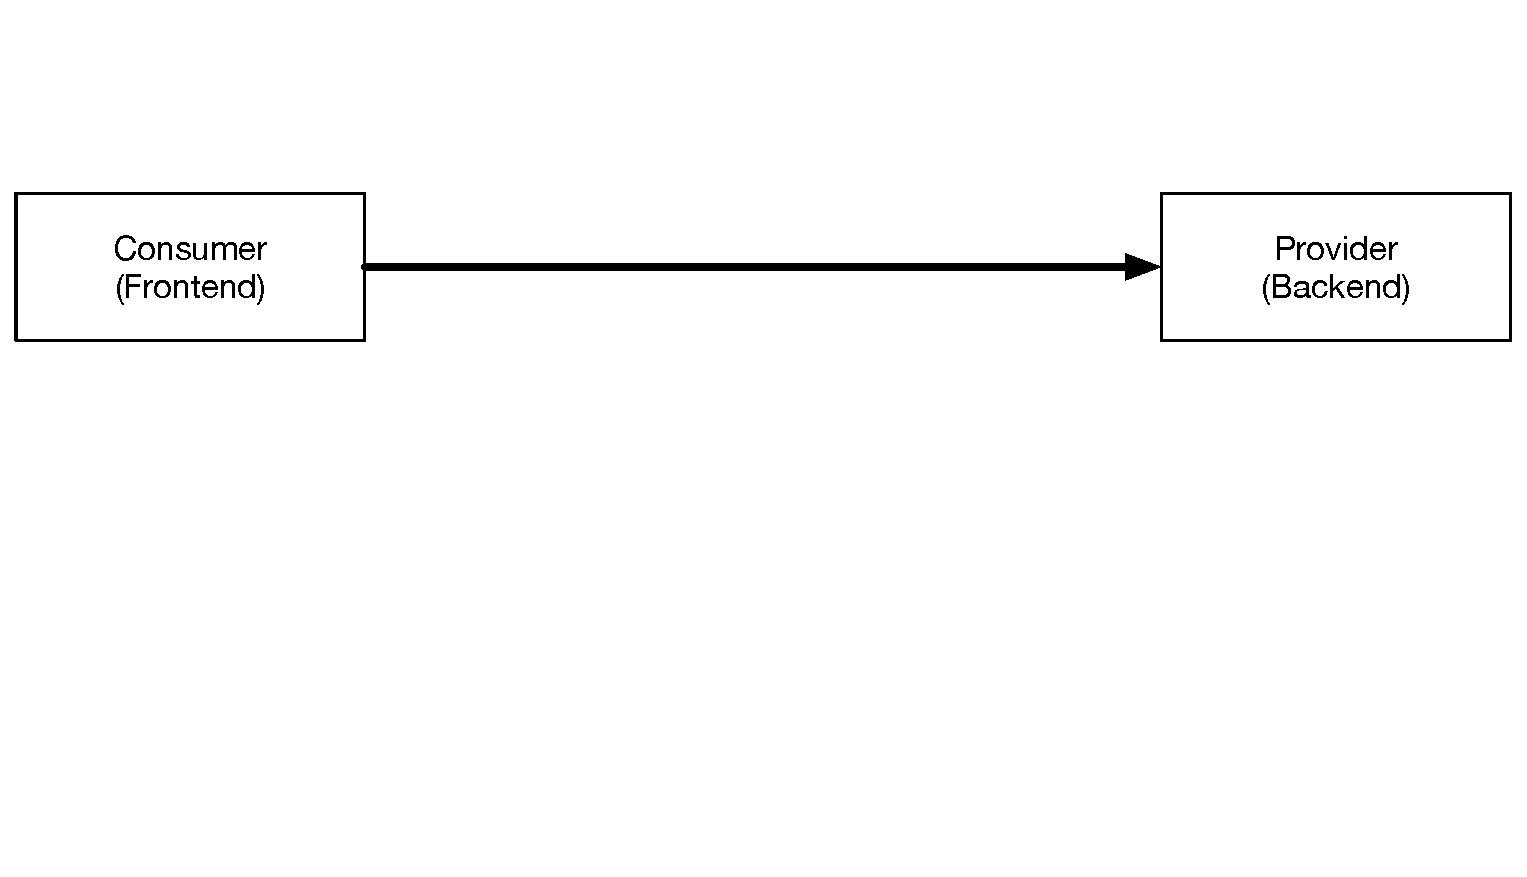
\includegraphics[width=\textwidth]{images/CDCT1.pdf}
}

\only<3>{
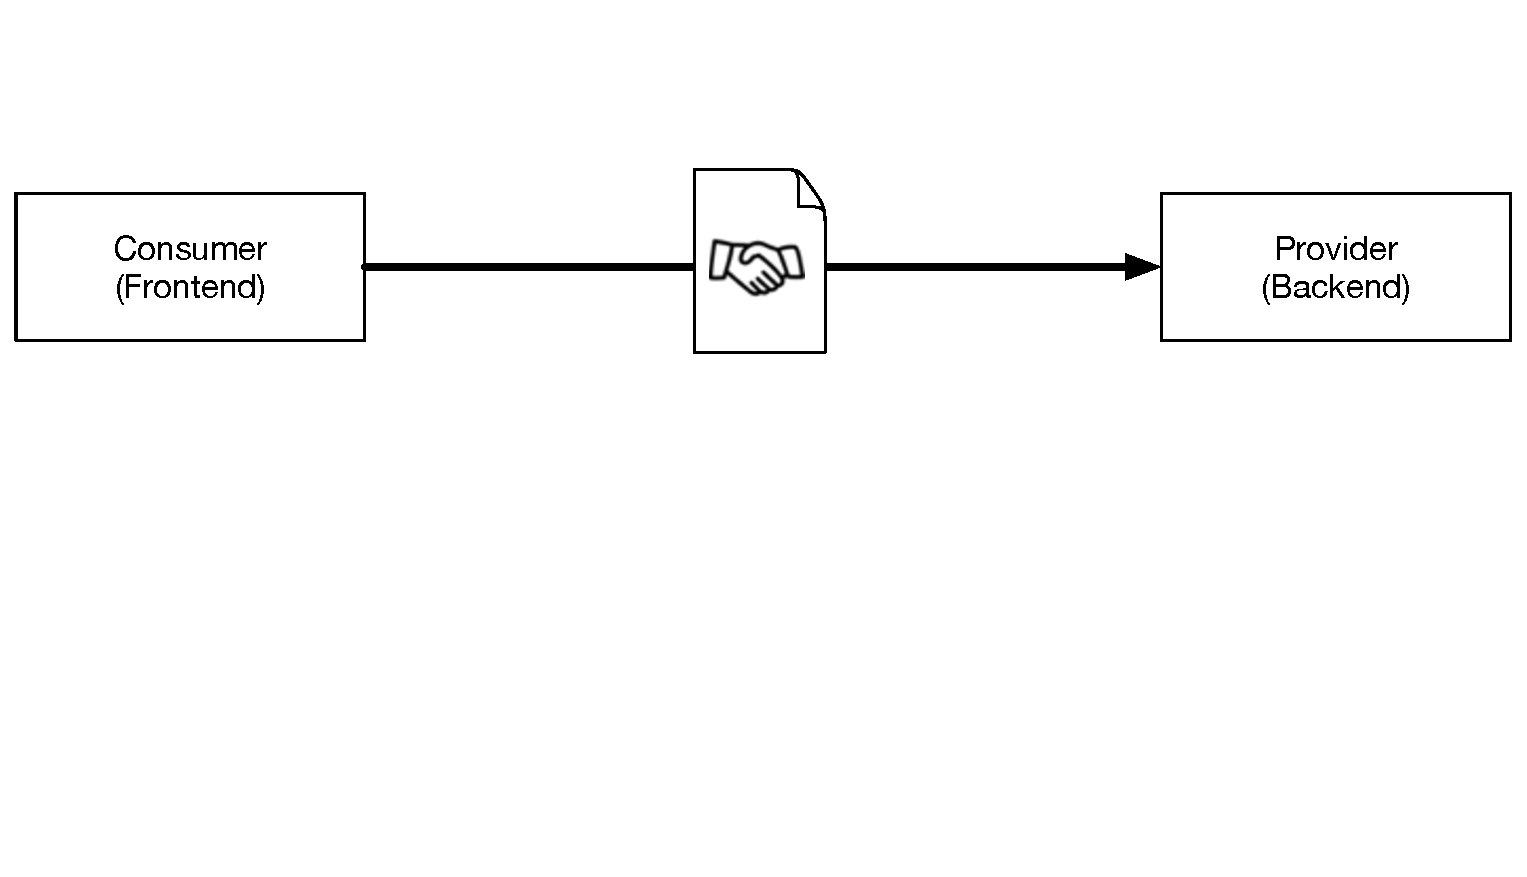
\includegraphics[width=\textwidth]{images/CDCT2.pdf}
}

\only<4>{
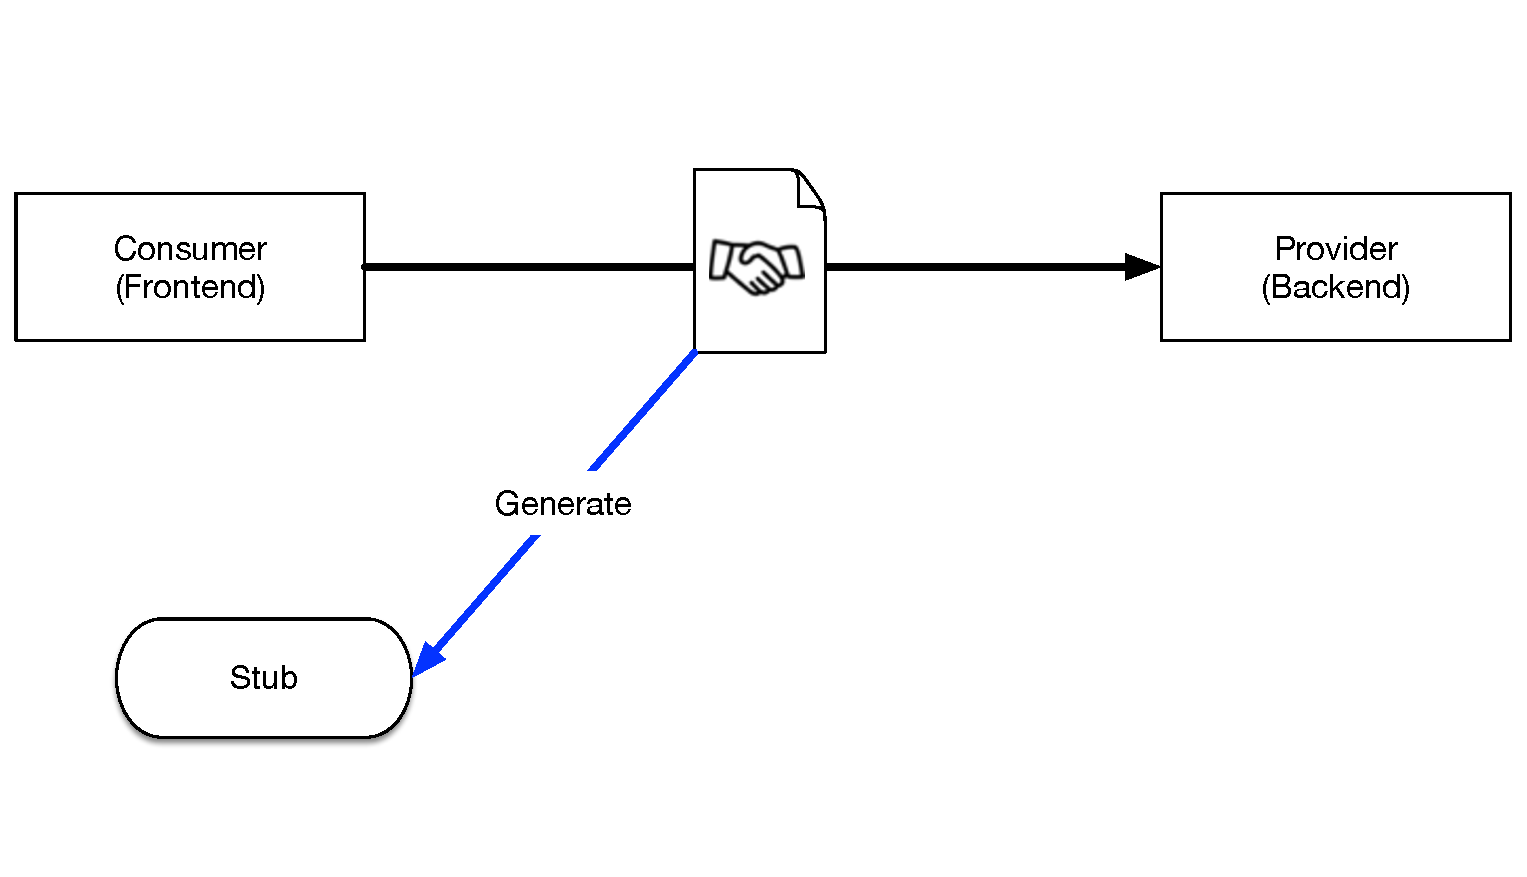
\includegraphics[width=\textwidth]{images/CDCT3.pdf}
}

\only<5>{
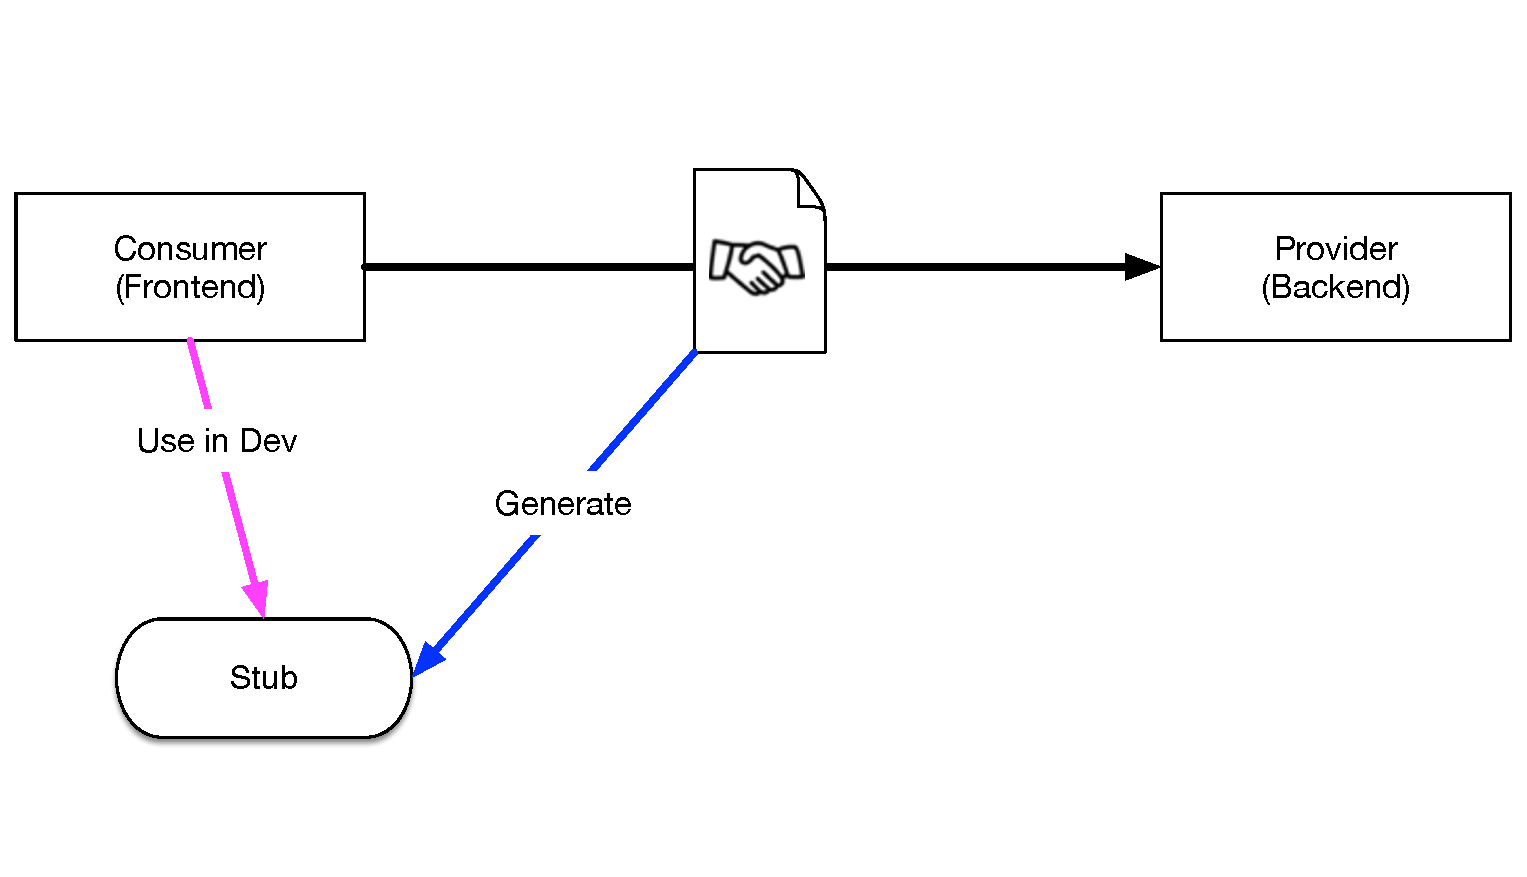
\includegraphics[width=\textwidth]{images/CDCT4.pdf}
}

\only<6>{
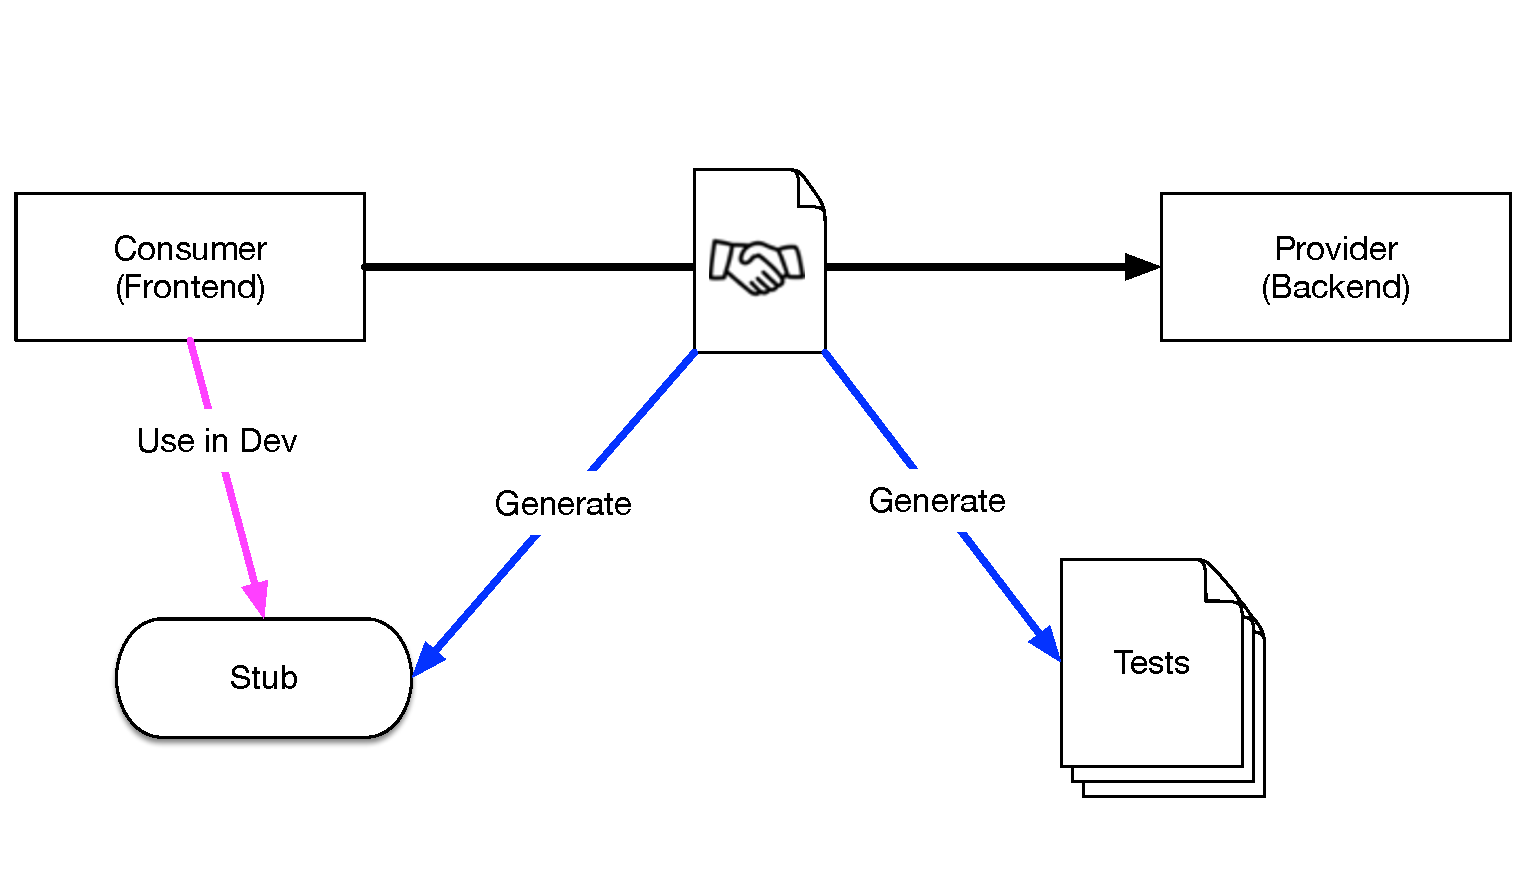
\includegraphics[width=\textwidth]{images/CDCT5.pdf}
}

\only<7>{
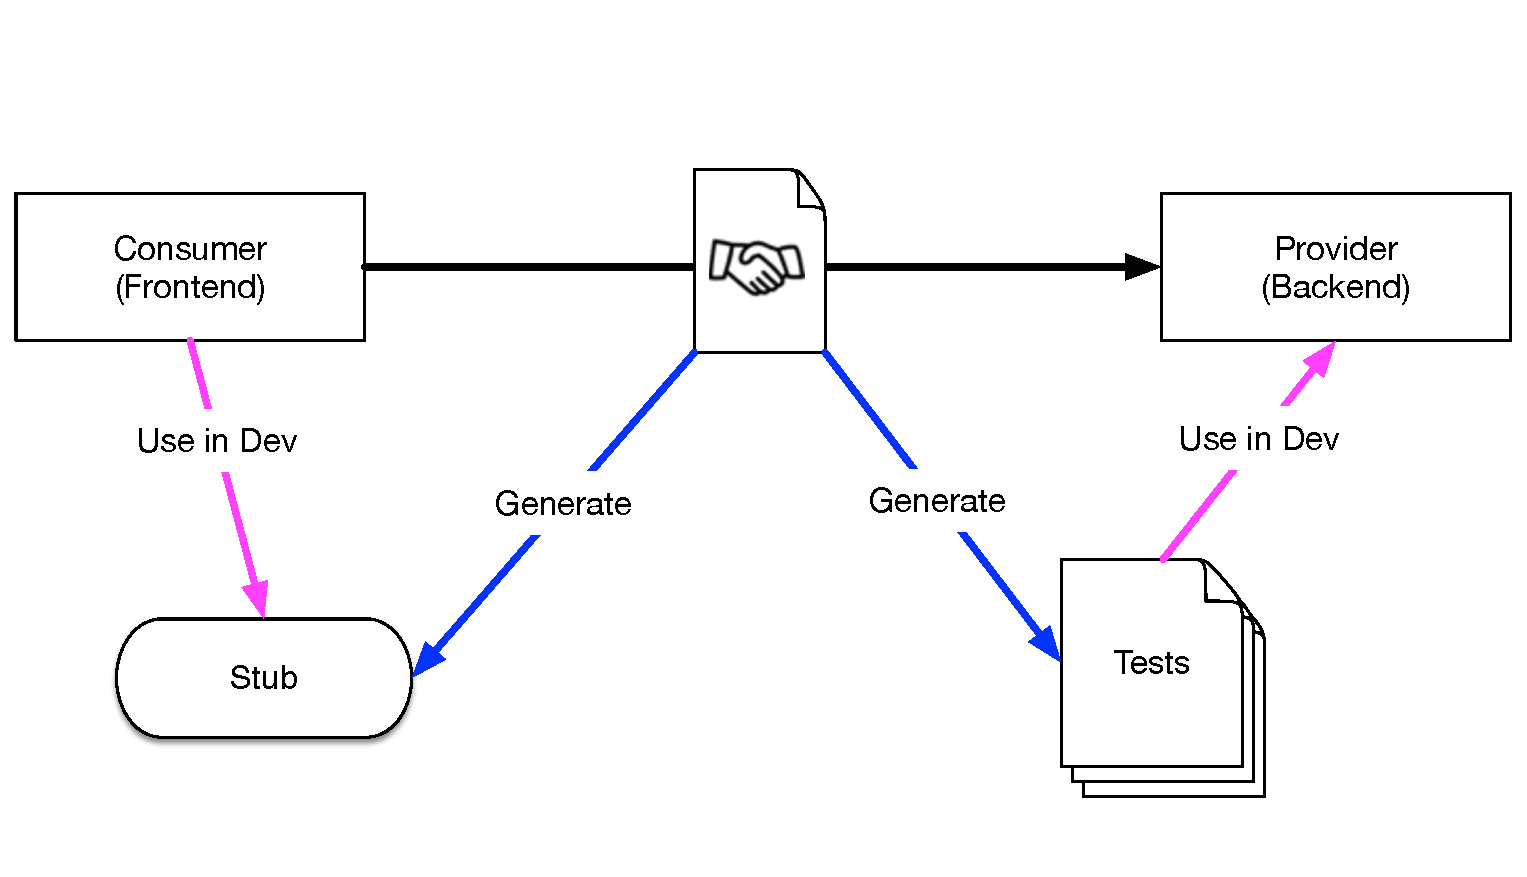
\includegraphics[width=\textwidth]{images/CDCT6.pdf}
}

\only<8>{
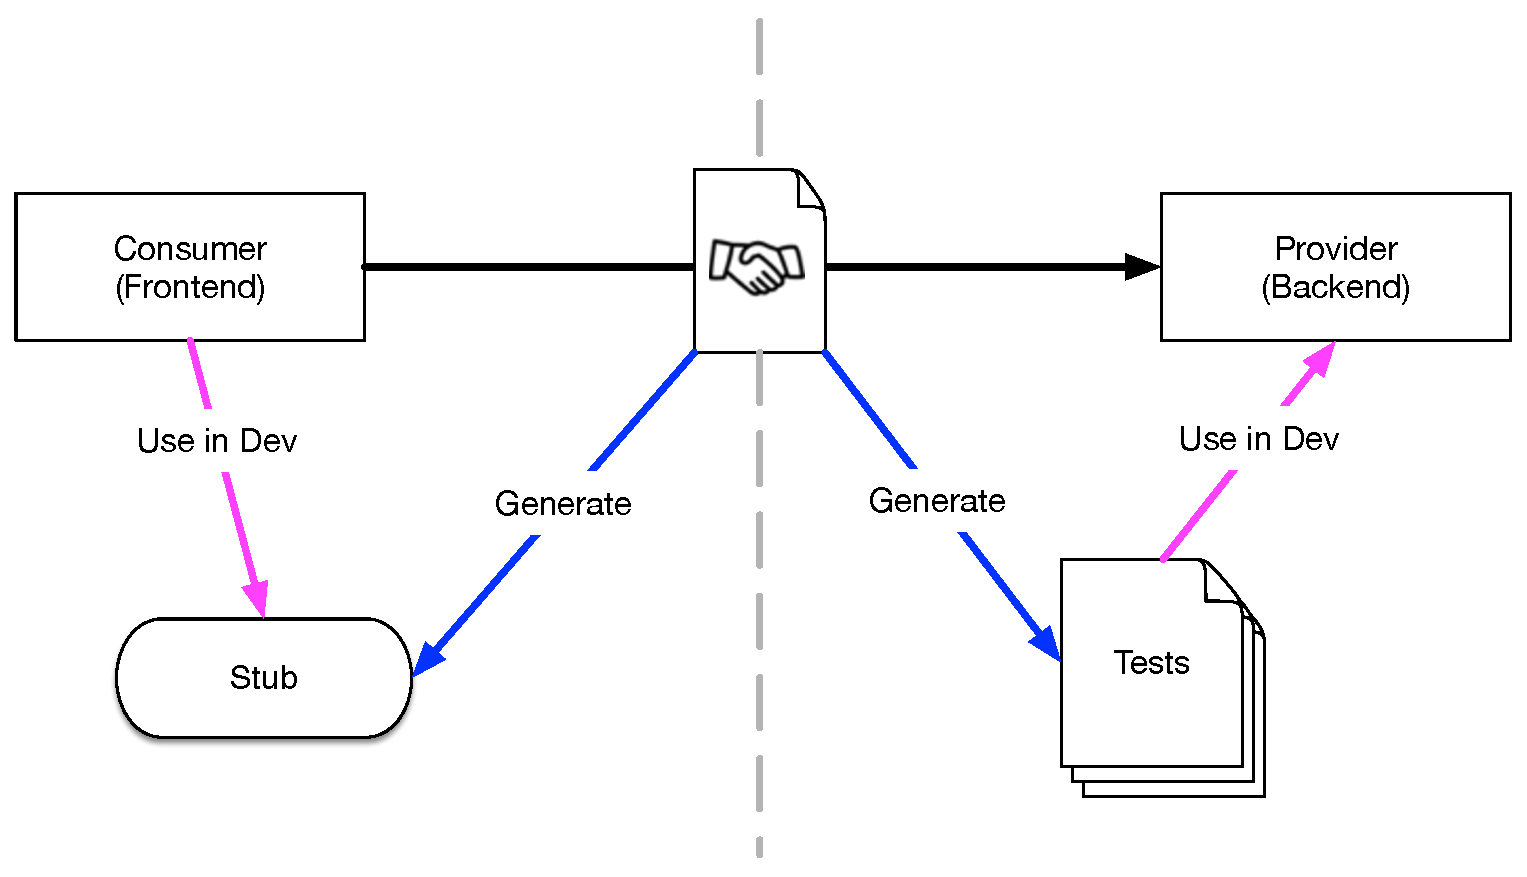
\includegraphics[width=\textwidth]{images/CDCT7.pdf}
}

\only<9>{
Problems:

\begin{itemize}
\item Contract testing is only as good as its contracts
\item Manual contract-writing can be tedious and even error-prone
\item Errors may only be discovered late in the process, when the backend implements some functionality and discovers that it does not match the contract
\item If contracts are too sparse, we miss out
\item If contracts are too verbose (or too many), testing takes too long
\end{itemize}
}

\end{frame}

\begin{frame}[fragile]{Back to Formal Models}
  \begin{itemize}[<+->]
  \item Often contracts are fairly simple, just mapping requests to replies
  \item What if some request only makes sense in a certain state?

  \item We need more information! Let's use \emph{State Machines}.
  \end{itemize}
\end{frame}


\begin{frame}[fragile]{Our ``formal model'' approach}

  \begin{itemize}[<+->]
  \item Describe the core domain interactions as a formal model
  \item Generate mocks for the frontend: Use the State Machine as an \emph{Acceptor}
  \item Generate tests for the backend: Use the State Machine as a \emph{Generator}
  \item Guarantee: All aspects of  the model are covered by tests and mocks
  \end{itemize}

\end{frame}


%%%%%%%%%%%%%%%%%%%%%%%%%%%%%%%%%%%%%%%%%%%%%%%%%%
\part{Examples}

\begin{frame}[fragile]{Acquire}
  \begin{center}
    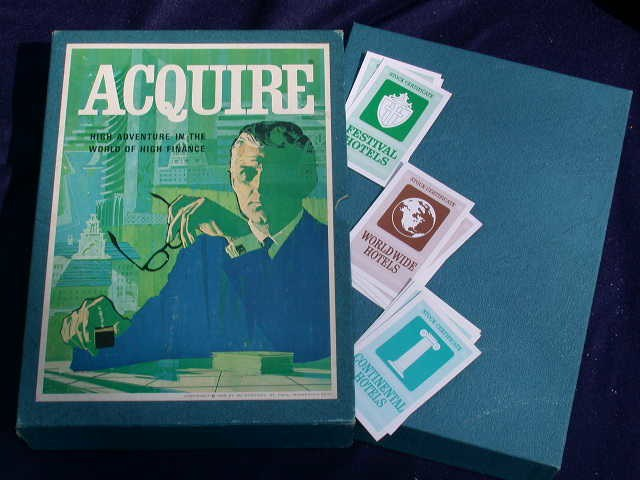
\includegraphics[height=.8\textheight]{./images/acquire-boardgame.jpg}
  \end{center}
\end{frame}

\begin{frame}[fragile]{Architecture - Backend}
  \begin{center}
    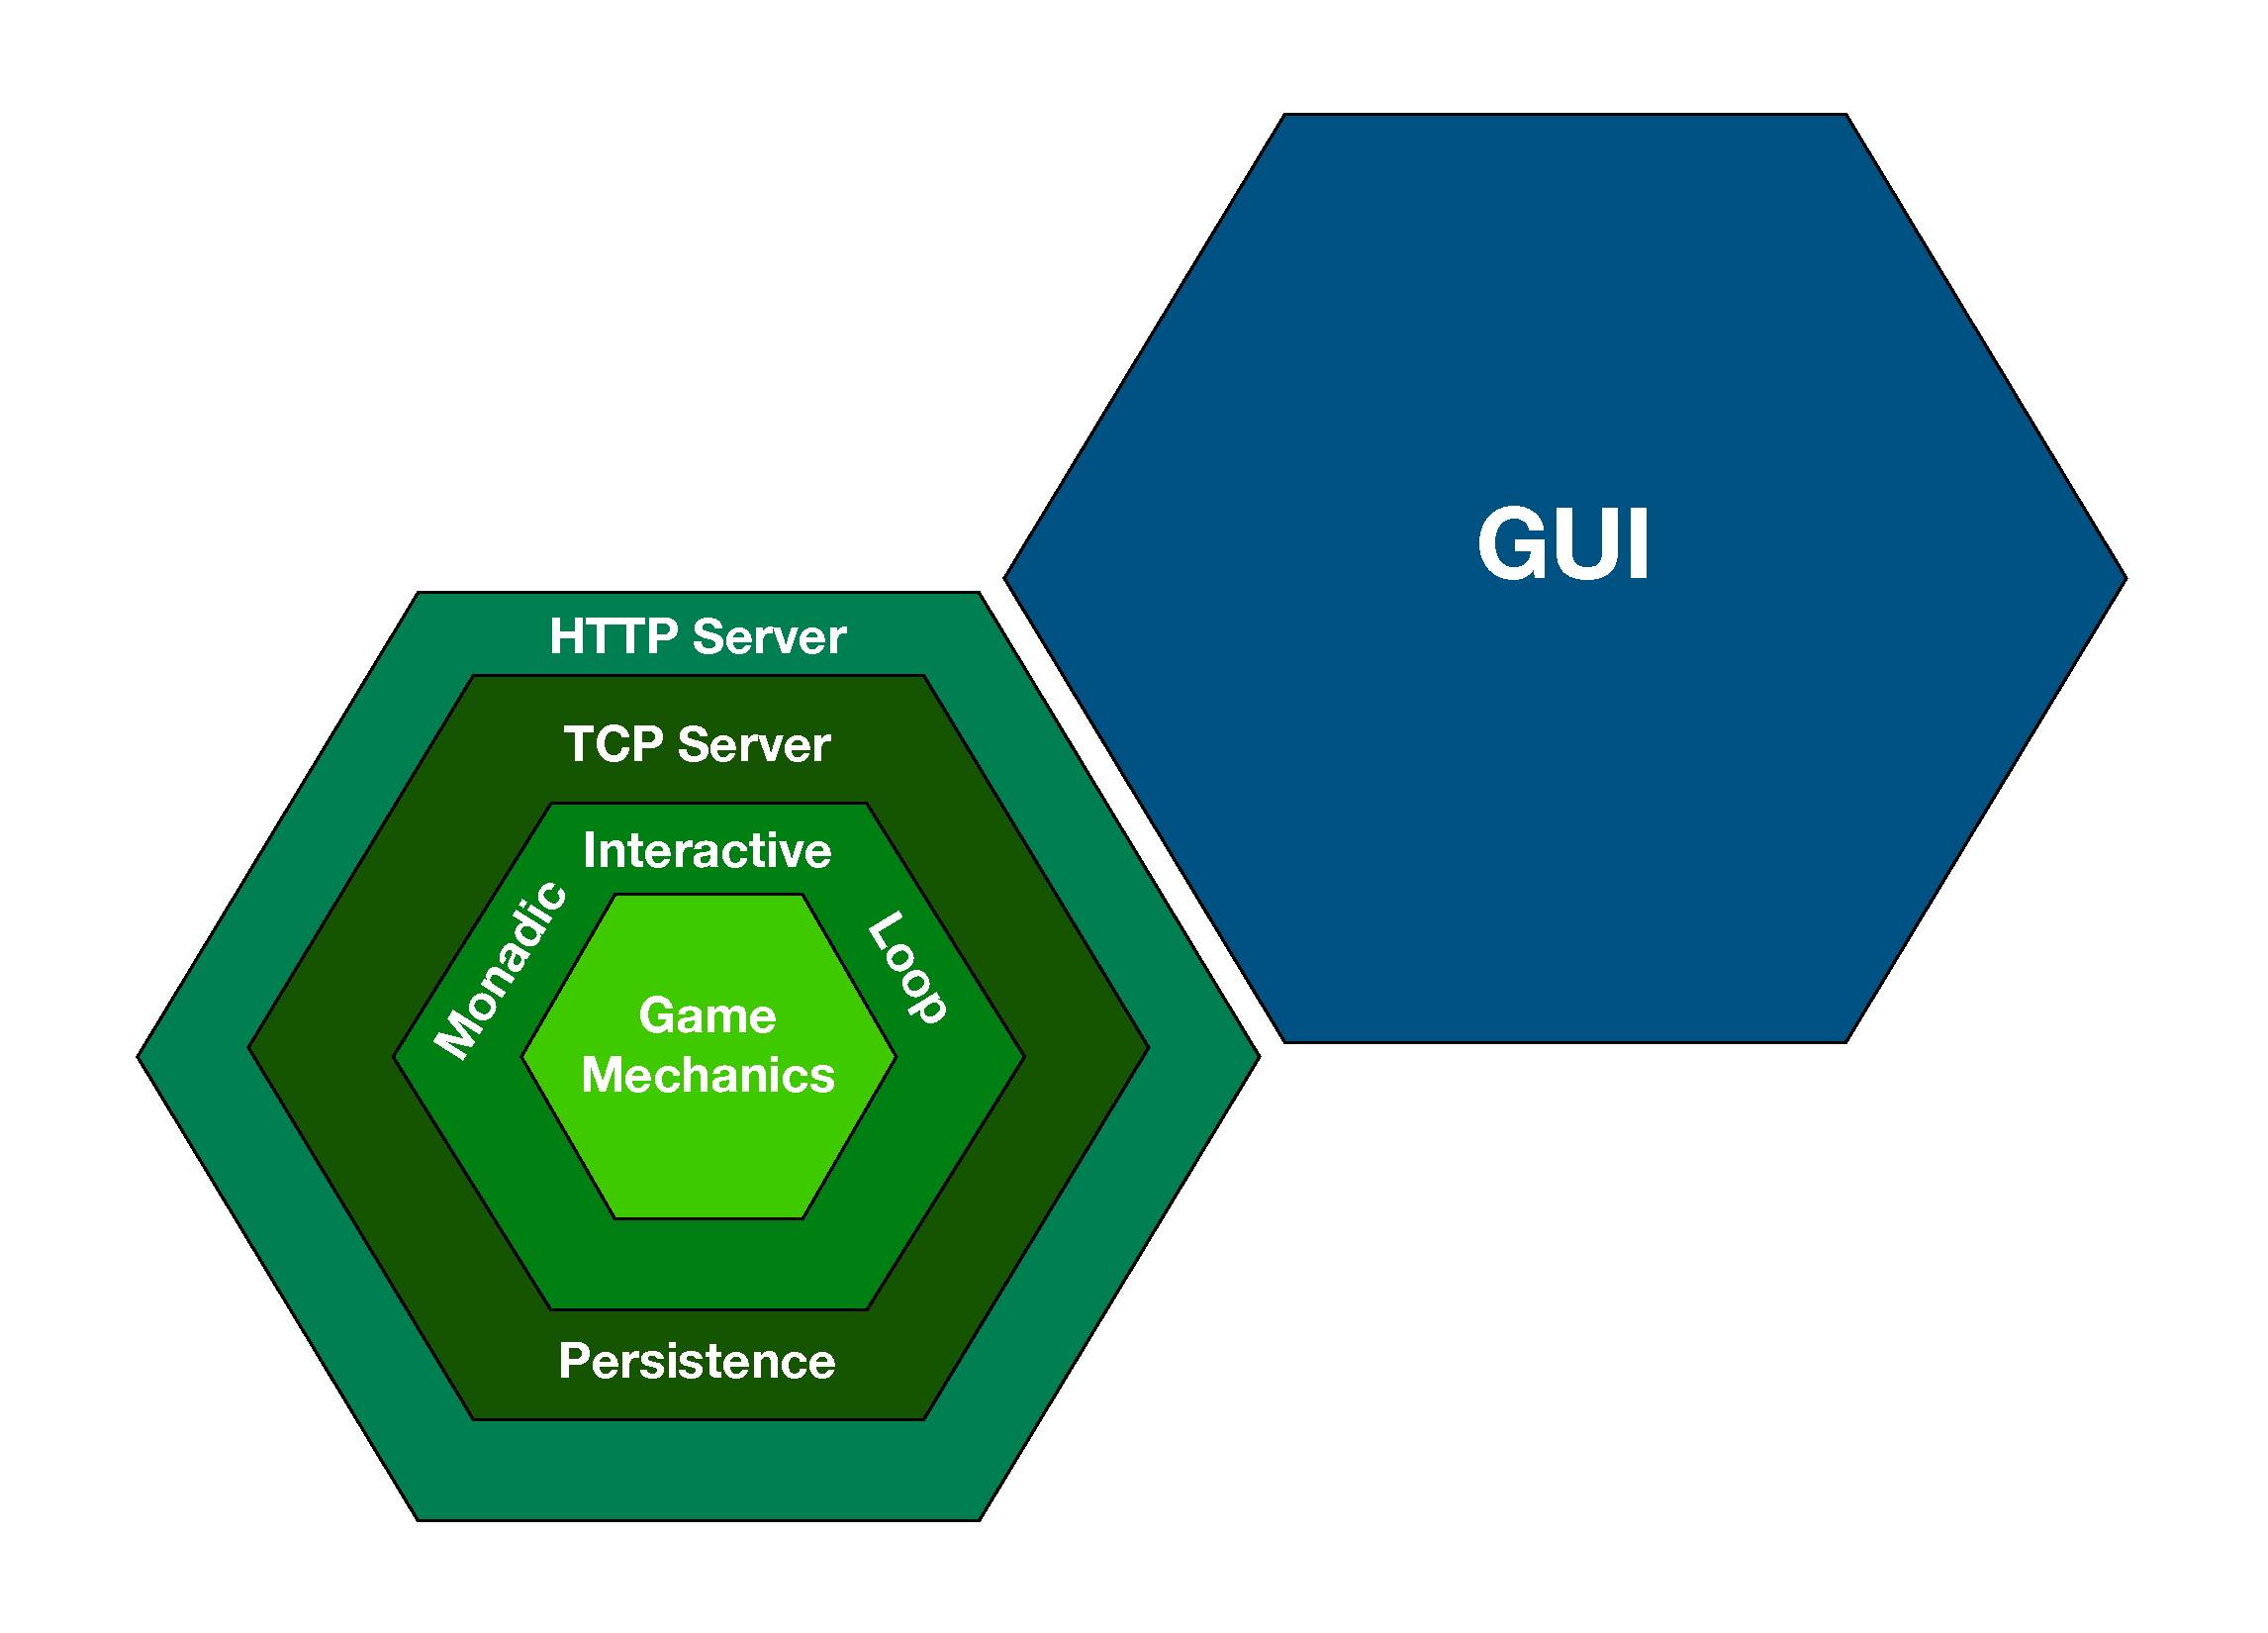
\includegraphics[height=.8\textheight]{./images/archi-back.pdf}
  \end{center}
\end{frame}

\begin{frame}[fragile]{Architecture - Frontend}
  \begin{center}
    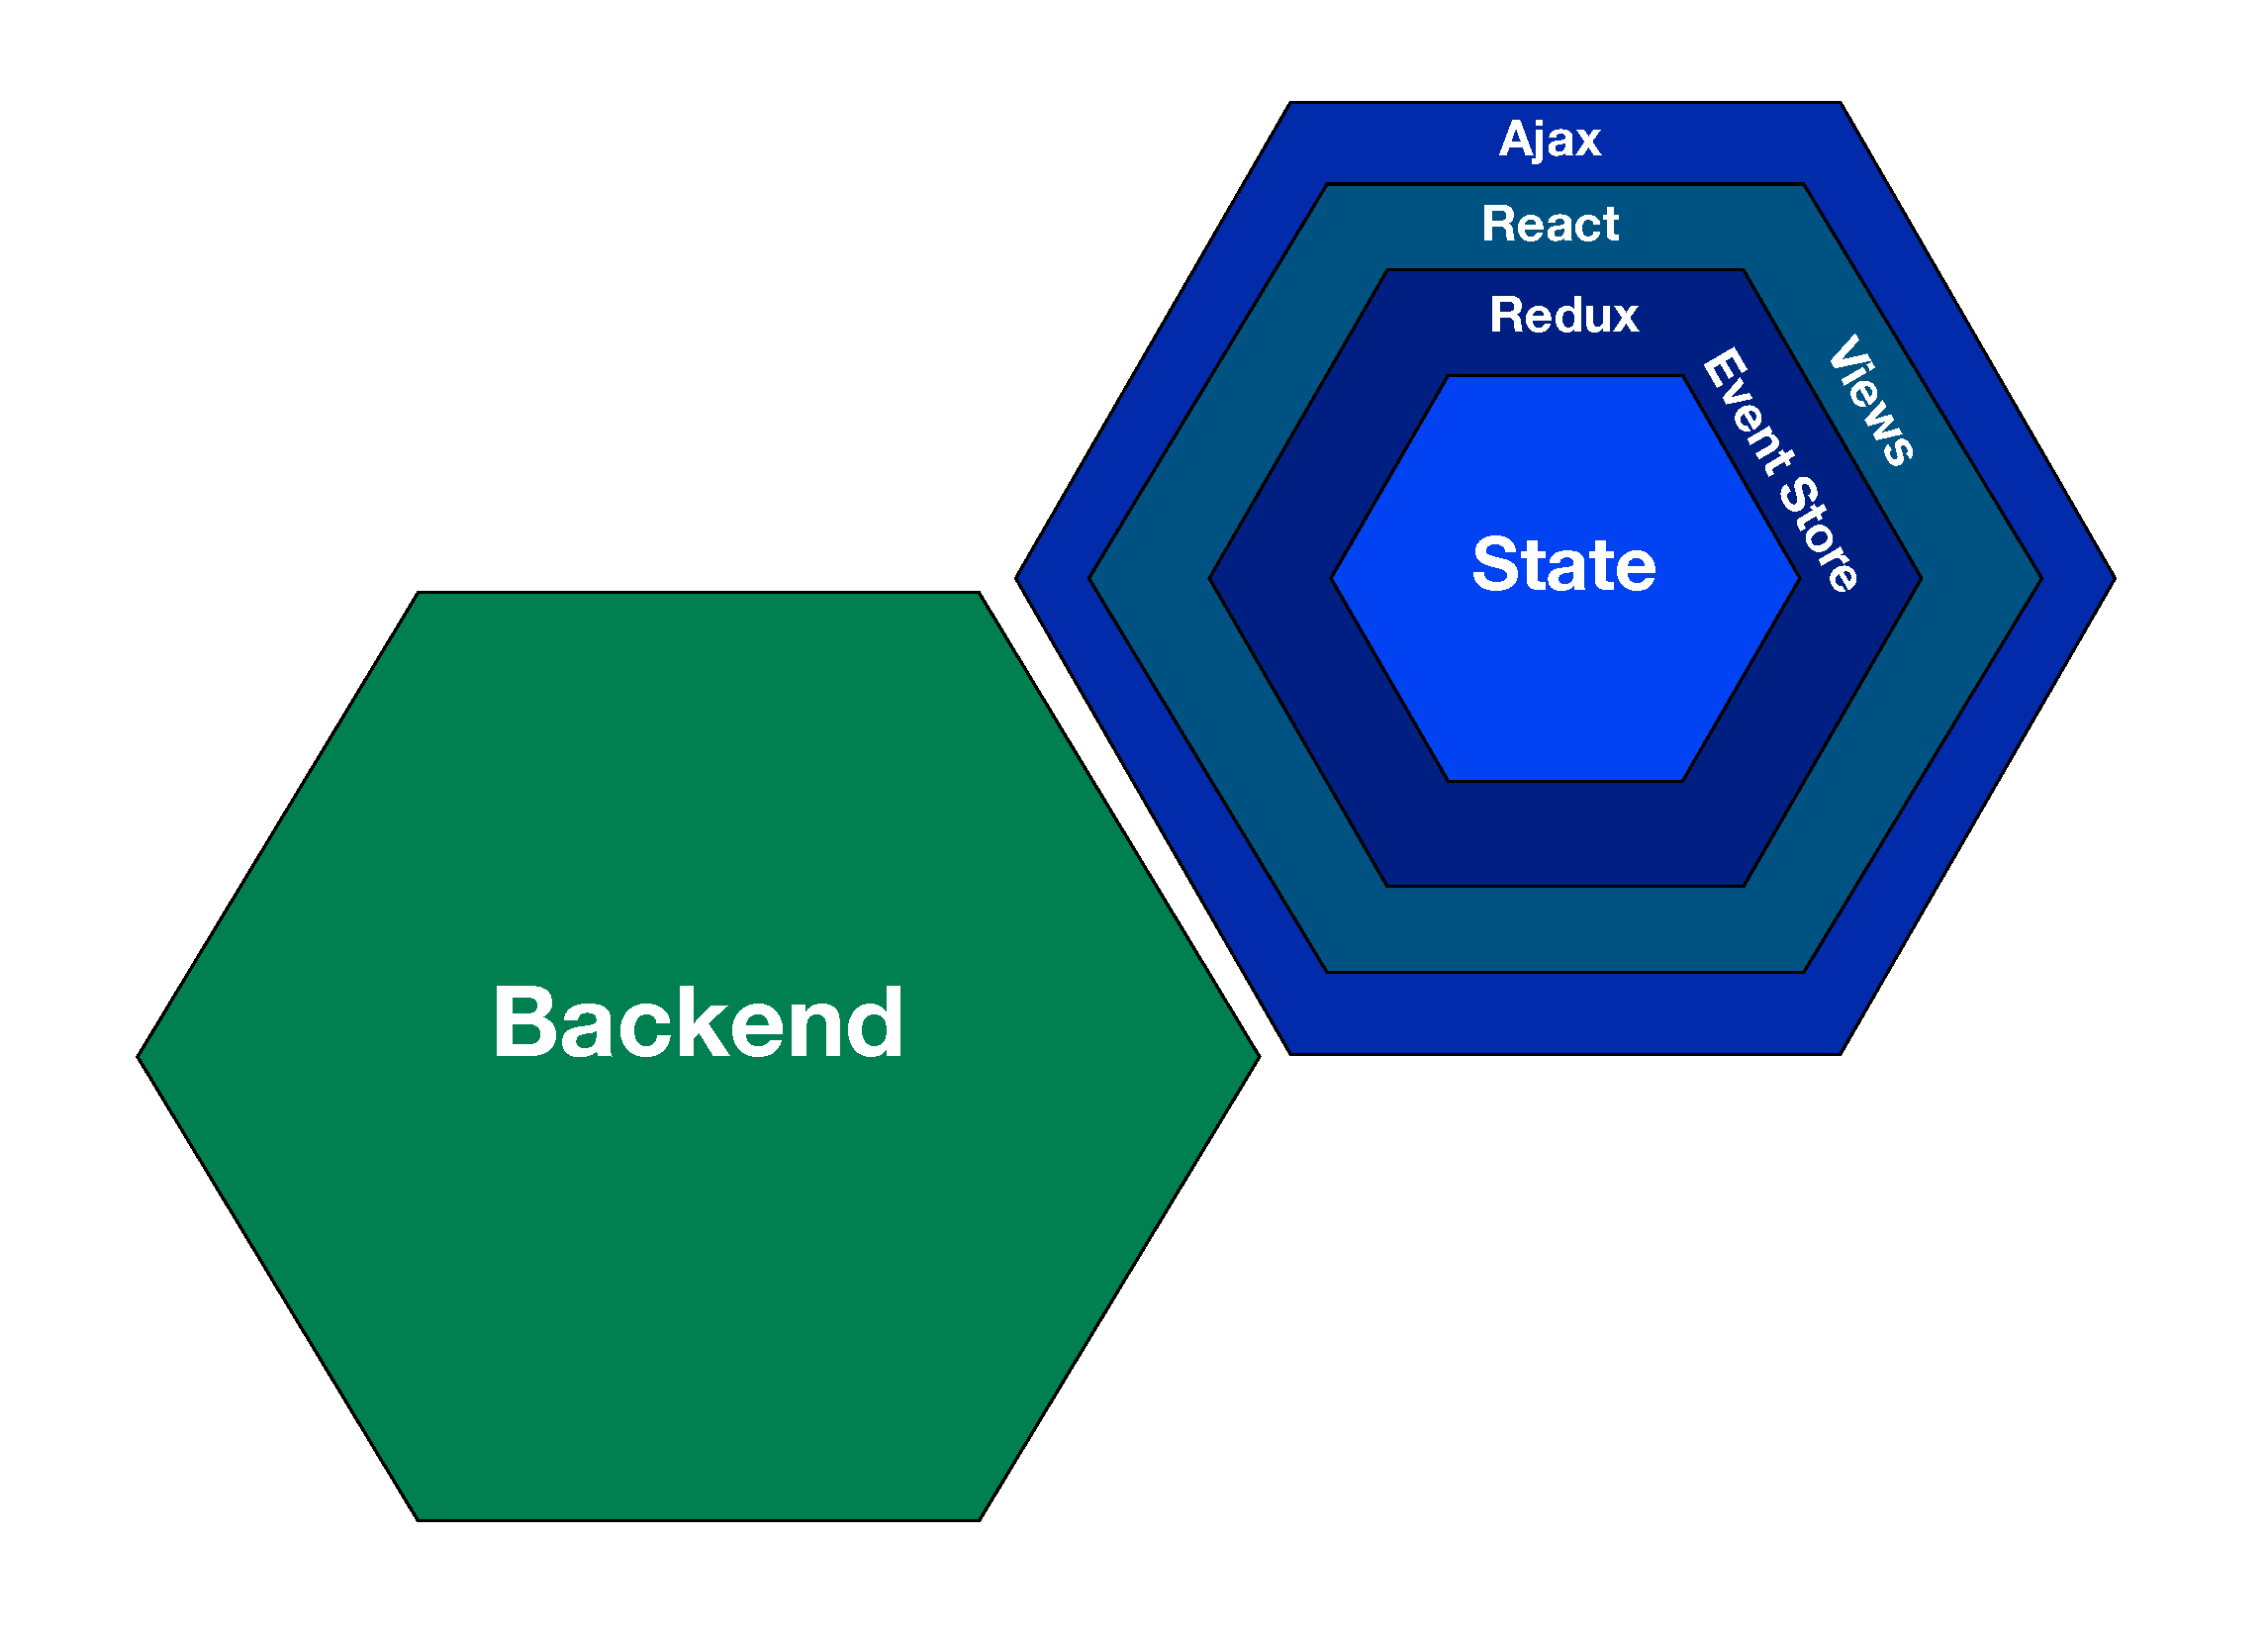
\includegraphics[height=.8\textheight]{./images/archi-front.pdf}
  \end{center}
\end{frame}

\begin{frame}[fragile]{The Code}
  \begin{center}
  \url{https://github.com/aleryo/homomorphic-event-sourcing}
  \end{center}
\end{frame}


%%%%%%%%%%%%%%%%%%%%%%%%%%%%%%%%%%%%%%%%%%%%%%%%%%
\part{Conclusion}

\begin{frame}[fragile]{Event Sourcing \& Formal Methods}
  \begin{itemize}[<+->]
  \item Building an\emph{Event Sourced} system yields opportunities to leverage more formal approaches to V\&V
  \item Modelling as a \emph{State Machine} over a \emph{Formal Language} is one possible approach
  \item Provides foundations to develop independent parts of the system and \emph{validate} their interaction
  \item It takes time and energy to devise and refine a model
  \end{itemize}
  \only<4>{
    \begin{block}{Event Sourcing as a Transduction}
      \[
        \begin{array}{c}
          \text{Command} \times \text{State} \rightarrow \text{Event} \times \text{State} \\
          \Updownarrow \\
          \text{State} \xrightarrow{\text{Command} \times \text{Event}} \text{State} \\
        \end{array}
      \]
    \end{block}
  }
\end{frame}

\begin{frame}[fragile]{Takeaways}
  \only<1>{\Huge \begin{quote} Plans are worthless,\\ but planning is everything \\ \textsc{\Large Dwight D. Eisenhower}\end{quote}}
  \only<2>{\Huge \begin{quote} Models are worthless,\\ but modelling is everything \\ \textsc{\Large Nicole \& Arnaud}\end{quote}}
\end{frame}

%%%%%%%%%%%%%%%%%%%%%%%%%%%%%%%%%%%%%%%%%%%%%%%%%%
\begin{frame}{Thank you very much!}

  ~\\[1em]
  \begin{block}{Arnaud Bailly}
        \begin{description}[Twitterxx]
        \item[E-Mail]  \href{mailto:arnaud@aleryo.com}{\texttt{arnaud@aleryo.com}}
        \item[Twitter] \href{http://twitter.com/NicoleRauch}{\texttt{@dr\_c0d3}}
        \item[Web] \href{http://aleryo.com}{\texttt{http://aleryo.com}}
        \item[Web] \href{http://symbiont.io}{\texttt{http://symbiont.io}}
        \end{description}
  \end{block}
  \begin{block}{Nicole Rauch}
    \begin{description}[Twitterxx]
    \item[E-Mail]  \href{mailto:info@nicole-rauch.de}{\texttt{info@nicole-rauch.de}}
    \item[Twitter] \href{http://twitter.com/NicoleRauch}{\texttt{@NicoleRauch}}
    \item[Web] \href{http://www.nicole-rauch.de}{\texttt{http://www.nicole-rauch.de}}
    \end{description}
  \end{block}
\end{frame}

%% https://i2.wp.com/thebiggamehunter.com/wp-content/uploads/2011/02/Acquire-3M-Sid-Sackson-11.jpg
